\section*{Exercice 4~: Spécification d'une construction d'une maison}

\subsection*{Questions 1 et 2}

\textit{Cf.} figures $1$ et $2$.

\begin{figure}[h!]
\begin{center}
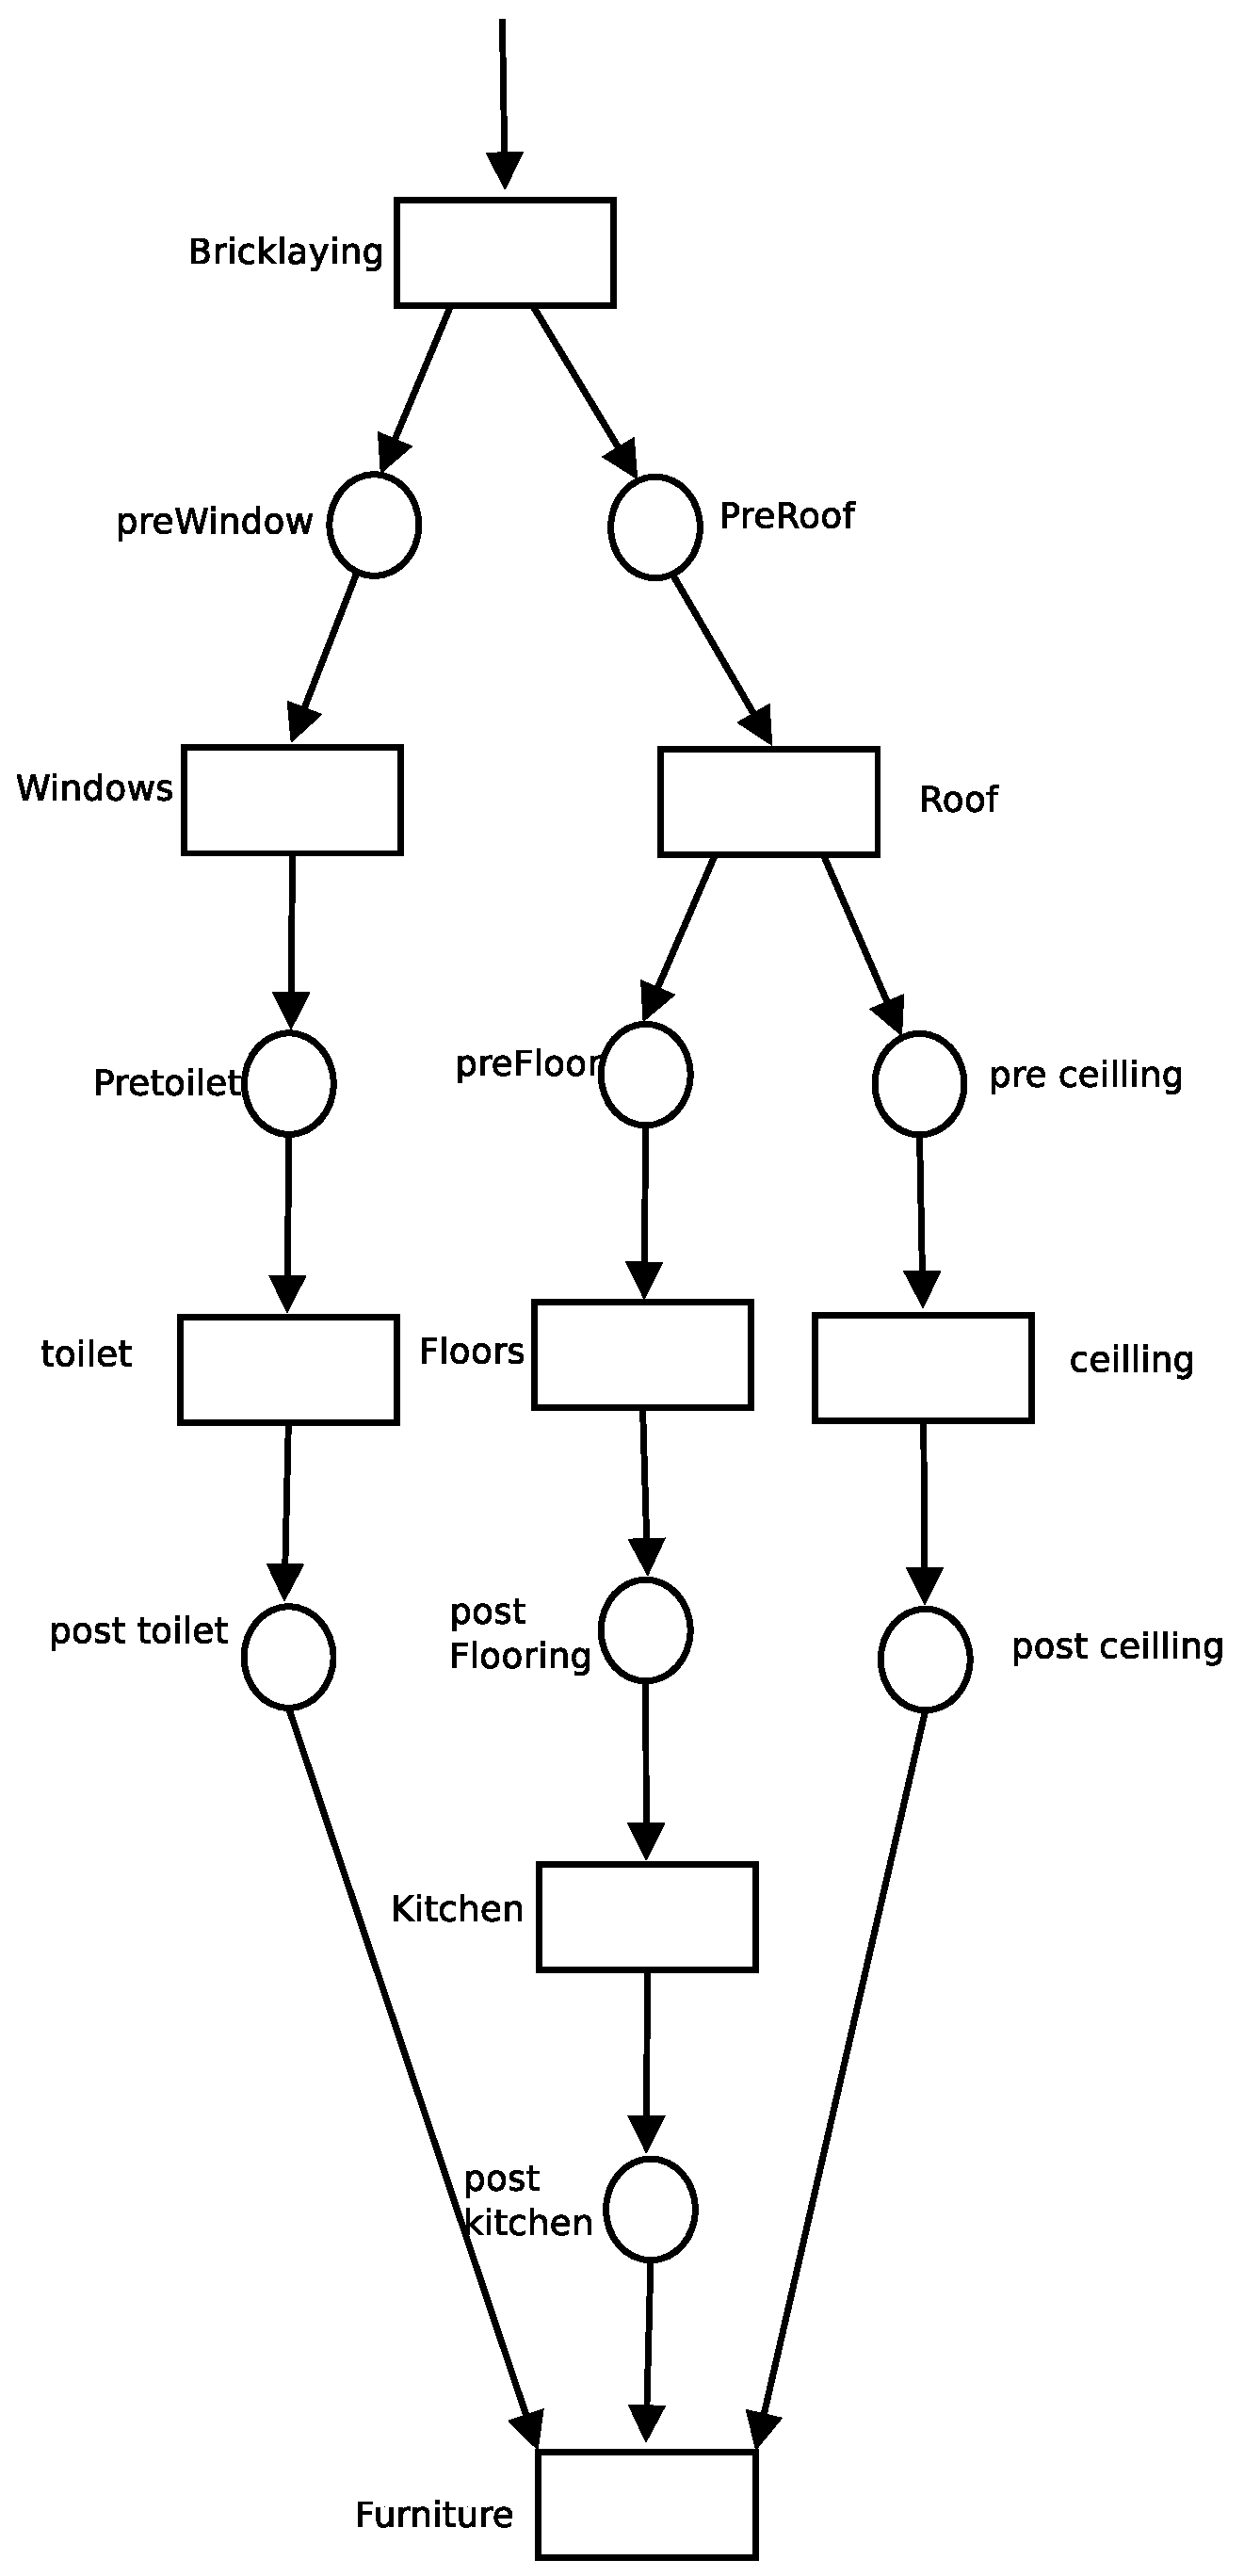
\includegraphics[height = 13cm]{exo41.eps} 
\caption{PT-net where each task is represented by a transition}
\end{center} 
\end{figure} 


\begin{figure}[h!]
\begin{center}
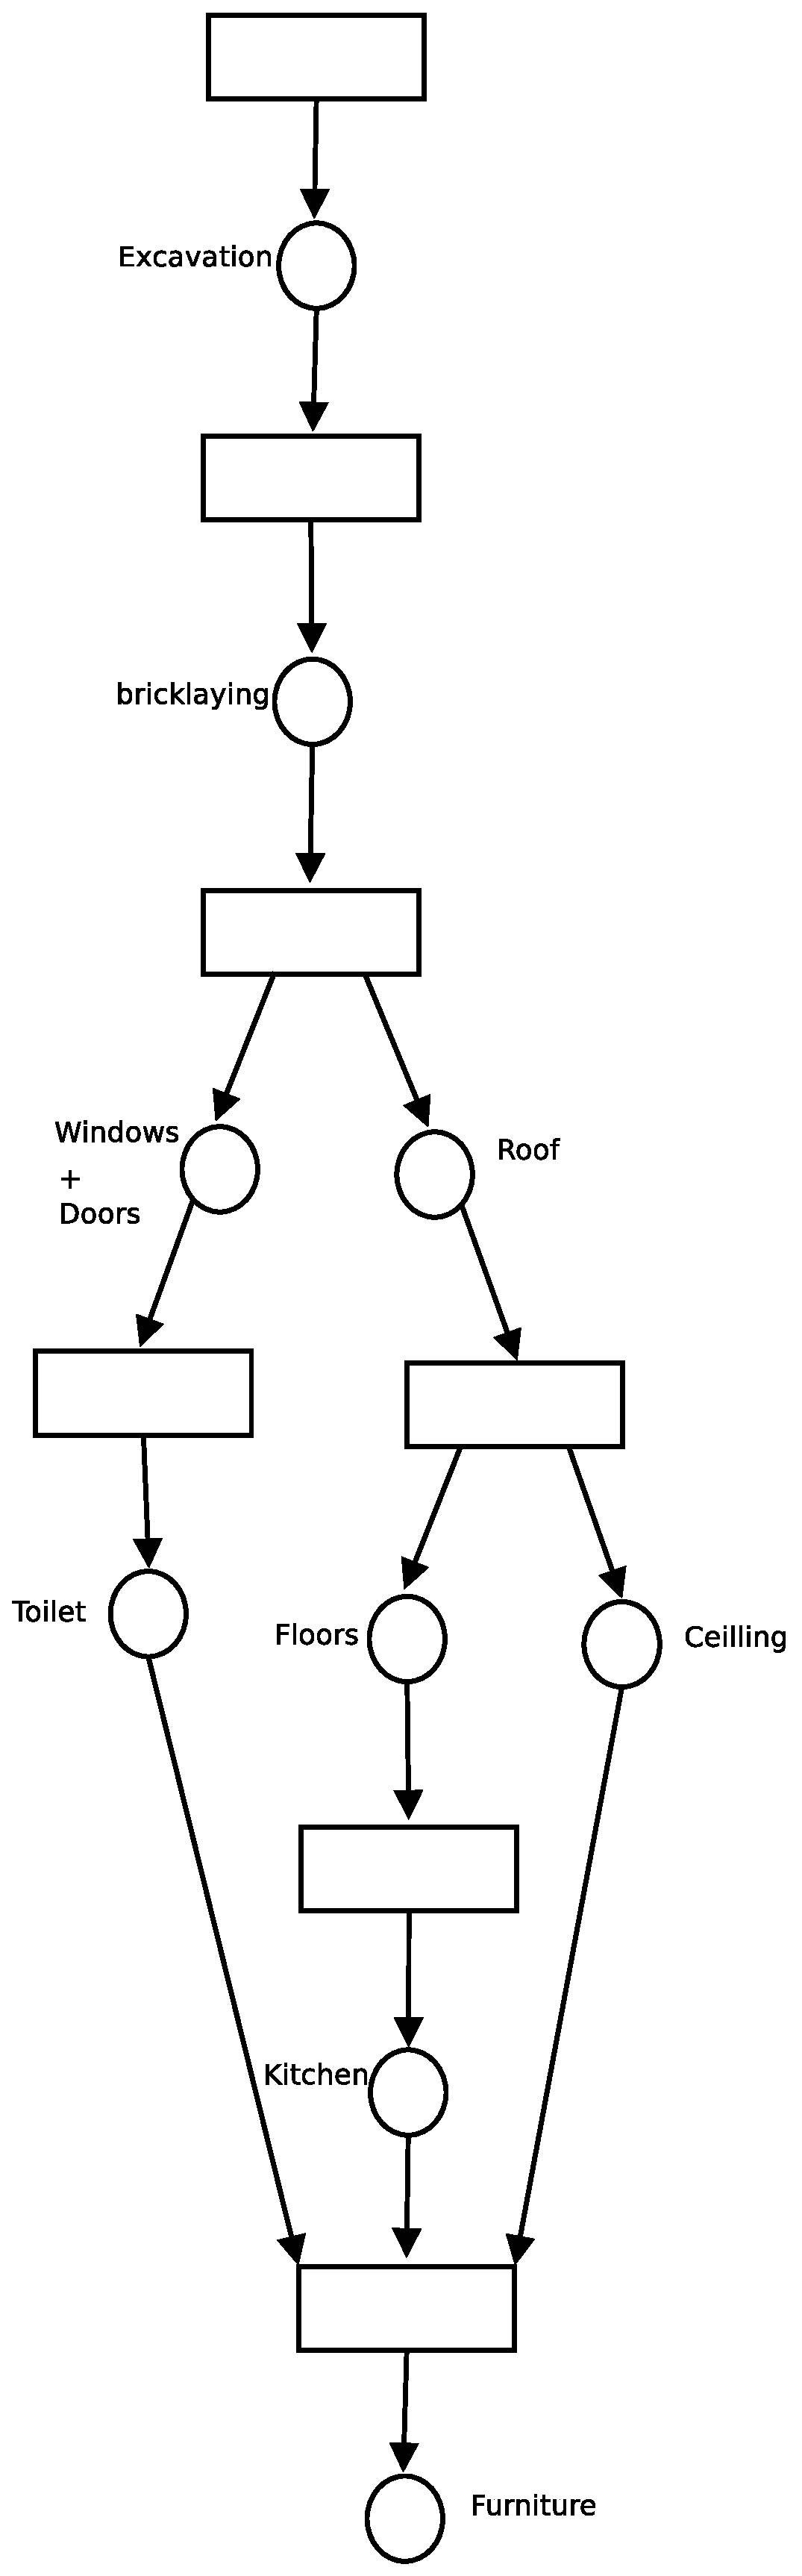
\includegraphics[height = 13cm]{exo42.eps} 
\caption{PT-net where each task is represented by a place}
\end{center} 

\end{figure}
\subsection*{Question 3}

Bien que les deux réseaux de pétri conservent la sémantique, le
deuxième semble plus naturel dans la mesure où l'on n'introduit pas
d'état artificiel d'entre-action. Modéliser les tâches par des places
convient donc mieux, les transitions servant à exprimer le passage
d'une tâche à l'autre, notamment la complétion d'une tâche.
